\chapter{\library{Lantern}: Data-driven Acoustic Echo Retrieval}\label{ch:lantern}

\marginpar{%
    \footnotesize
    \textbf{Keywords:} Acoustic Echo Retrieval, TDOA Estimation, Supervised Learning, Deep Learning, Regression.
    \\\textbf{Resources:}
    \begin{itemize}
        \item \href{aoeu}{Paper}
        \item \href{aoeu}{Code}
        \item \href{aoeu}{Poster}
    \end{itemize}
}
\newthought{Synopsis} \synopsisChLantern

\mynewline
The material presented in this chapter is part of the previously published work~\cite{di2019mirage} and of a technical report for HONDA\textregistered~\citeonly{di2019honda}.

\section{Introduction}
The following sections gives a review of machine learning theory knowledge required by the reader in order to understand the implementations related to machine learning in this chapter.
The review includes basic theory behind neural networks and deep learning including layer-types, optimization and loss functions, as well as aspects related to training on \RIRdef/.
This section also gives a brief review of why and how to use autoencoders.

\subsection{Supervised Learning}

\newthought{End-to-end learning}
\newthought{2-stage learning}

\newthought{Virtually Supervised Learning}

\subsection{Neural Networks}

\newthought{Convolutional Neural Networks and Deep Learning}

\subsection{For the \RIR/ and the \AER/?}


\section{Proposed Learning-based \AER/}

\subsection{Simple Case: $\numEchs = 2$}

Our approach is to train a deep neural network (DNN) on a dataset simulating the considered close-surface scenario.
We model the problem as multi-target regression, with \textit{interaural level difference} (ILD)
and \textit{interaural phase difference} (IPD) as input features, and $V \in \mathbb{R}^3$ as output parameters.
ILD and IPD features are defined in the frequency domain as follows:
\begin{equation}
\label{eq:mirage:features}
\begin{cases}
ILD(f)  =& \tfrac{1}{T} \sum_{t=1}^T \log{\mid \frac{M_2(f,t)}{M_1(f,t)} \mid } \\
IPD(f)  =& \tfrac{1}{T} \sum_{t=1}^T \frac{M_2(f,t)/ \mid M_2(f,t) \mid }{M_2(f,t) / \mid M_1(f,t)  \mid}\\
\end{cases}
\end{equation}
More precisely, the input of the network is
$\mathbf{x} = [ILD,$ $\operatorname{Re}(IPD)], \operatorname{Im}(IPD)]$, where $\operatorname{Re}$
and $\operatorname{Im}$ denote real and imaginary part operators, respectively.
Note that for the IPD, the frequency $f=0$ is discarded because it is constant for every observation.
In general, the mapping between $V$ and the proposed feature is not unique.
In particular, this happen when $\tau_2^1 = \tau_1^1$.
In order to avoid this, we preventively pruned all the entries
with $| \tau_2^1 - \tau_1^1 | < 10^{-6}$ from the dataset.

We use a simple fully-connected DNN architecture consisting of a $D$-dimensional input layer,
a $3$-dimensional output layer, and 3 fully connected hidden layers with respective input
sizes $500$, $300$ and $50$. Rectified linear unit (ReLU)
activation functions are used except at the output layer,
and each hidden layer has a dropout probability $p_\text{do} = 0.3$.
We use the mean square error loss function for training and the Adam optimizer \cite{kingma2014adam}.
The normalized root mean square error (nRMSE) is taken as validation
metric\footnote{The nRMSE takes values between $0$ (perfect fit) and $\infty$ (bad fit).
If it is equal to $1$, then the prediction is no better than a constant.}.
The network is manually tuned on a validation set to find the best combination of number of hidden layers, their sizes and $p_\text{do}$.
Once time delay estimates $\hat{V}$ are returned by the DNN, they are converted to synthetic
local angular spectra and passed to $\Psi_\text{SRP}$ (See Sec. \cref{subsec:mirage:2D-SSL})
together with the relative positions of true and image microphones which are assumed known.
We call this algorithm MIRAGE. The synthetic local angular spectra consist of Gaussians
centered at $\hat{V}$ and with variances equal to the prediction errors made by
the DNN on the validation set.

\section{Robust learning for the case $\numEchs = 2$}


The neural network follows the convolutional neural network (CNN) architecture in Figure~\ref{fig:cnn}, which is the one also used in \cite{Nguyen2018} and similar to the one used in \cite{Chakrabarty2017}. It consists in two convolutional modules made of one-dimensional convolutional layer (1DConv) followed by max-pooling along the frequencies, followed by rectified linear unit (ReLu) activation function and batch-normalization.
The second part consists in a cascade of fully connected feed-forward (FF) layers.
Note that dimension of the input is re-arranged so that the second dimension is considered as channel for the 1DConv. After each layer a dropout probability $p_\text{do} = 0.3$ is applied.

The proposed novel loss function is the negative Student-T log-likelihood, which is implemented as follows:

\begin{equation}
\begin{split}
\mathcal{L}(\Theta) =& \sum_{x \in B} \sum_{t \in V}\ \dfrac{1}{2} \log (\nu_t\pi_t)
                        + \dfrac{1}{2} \log(\lambda_t^2)
                        - \log  \Gamma \left( \dfrac{\nu_t+1}{2} \right)\\
                    &    + \log  \Gamma \left( \dfrac{\nu_t}{2} \right)
                        + \dfrac{\nu_t+1}{2}
                        \log \left( 1  + \dfrac{\norm{\mu_t, x_i)}}{\nu_t \lambda_t^2} \right)\\
\end{split}
\end{equation}

where $\Theta$ are the CNN parameters and $\Gamma$ is the Gamma function. The summation over $i$ corresponds to the sum among of all the sample $x$ of the batch $B$. and the summation over $t$ corresponds to the sum among the three quantities in V (TDOA, iTDOA, TDOE). It follows that for each each input the network will return the parameters of 3 Student-T distribution ($\mu_t, \nu_t, \lambda_t$) for each variable $t = { \text{TDOA}, \text{iTDOA}, \text{TDOE} }$. Hereafter we denote with $V_{\mathcal{ST}}$ the set of the 9 network outputs.

We use the Adam optimizer ant the normalized root mean square error (nRMSE) is taken as validation metric (see Section~\ref{subsec:eval_synth_tdoa}). The network is manually tuned on a validation set to find the best combination of number of hidden layers and their sizes

Once an estimate $\hat{V_\mathcal{ST}}$ of the parameters of the 3 distribution is returned by the CNN, they are converted to synthetic local angular spectra and passed to an SRP-PHAT method together with the relative positions of true and image microphones which are assumed known. We call this algorithm MIRAGE. The synthetic local angular spectra consist of Student-t distribution with parameters $\mu, \nu$ and $\lambda$.

For training and validation of the CNN we generate many random shoe-box room configurations using the software presented in \cite{schimmel2009fast}. This software implements both the image-method for simulating reflections and a ray-tracing algorithm for diffusion. Room widths are uniformly drawn at random in $[3, 9]$ m, heights in $[2, 4]$ m. Random source/microphones positions and absorption coefficients for the 6 surfaces are used, respecting the close-surface scenario. In particular, the microphones are at most $30$ cm from the close-surface, placed $13$ cm from each other, the absorption coefficients of the other walls are uniformly sampled in $(0.5, 1)$ and the one of the close-surface is in $(0, 0.5)$. The same realistic diffusion profile \cite{gaultier2017vast} is used for all surfaces. Around $20,000$ audio scenes are generated this way, yielding reverberation times ($RT_{60})$ between $20$ ms and $250$ ms.

For training and validation, the RIRs are convolved with 1 sec of white-noise with additional noise with SNR in $(0,20)$ dB.
All signals and RIRs are sampled at $16$ kHz. The STFT is performed on $1024$ point with $50\%$ overlap. Finally the features are computed as in~\eqref{eq:features} yielding a vector of size $D = 1534$ for each observation.
While we validate the CNN on a portion of the dataset in a \textit{holdout} fashion, the test is conducted on 200 new RIRs convolved with both speech utterances. This set is generated similarly to the training and validation sets. Moreover the recordings are perturbed by external white noise as in the training set. The speech signals are normalized speech utterances of various lengths (from $1$ s to $6$ s), randomly selected from the TIMIT corpus.
A re-implement version of SRP-PHAT is used to aggregate local angular spectra obtained from the DNN's output and as a baseline. However the original MATLAB code for SRP-PHAT can be found at \url{http://bass-db.gforge.inria.fr/bss_locate/}. A sphere sampling with $1$ degree resolution and coordinates $\theta \in [-179, 180]$ and $\phi \in [0, 90]$ degrees is used for the DOA search.



For training and validation of the DNN we generate many random, shoe-box room configurations using the software presented in \citeonly{Schimmel2009}.
This software implements both the image-method for simulating reflections and a ray-tracing algorithm for diffusion.
Room widths are uniformly drawn at random in $[3, 9]$ m, heights in $[2, 4]$ m.
Random source/microphones positions and absorption coefficients for the 6 surfaces are used,
respecting the close-surface scenario. In particular, the microphones are at most $30$ cm from the close-surface,
placed $10$ cm from each other, the absorption coefficients of the other walls are
uniformly sampled in $(0.5, 1)$ and the one of the close-surface is in $(0, 0.5)$.
The same realistic diffusion profile \citeonly{gaultier2017vast} is used for all surfaces.
Around $90,000$ audio scenes are generated this way, yielding reverberation times ($RT_{60})$ between $20$ ms and $250$ ms.

For training and validation, the RIRs are convolved with 1 sec of white-noise (wn) with no additional noise.
All signals and RIRs are sampled at $16$ kHz. The STFT is performed on $1024$ point with $50\%$ overlap.
Finally the features are computed as in~\eqref{eq:mirage:features} yielding a vector of size $D = 1534$ for each observation.
While we validate the DNN on a portion of the dataset in a \textit{holdout} fashion, the test is conducted on 200 new RIRs convolved with both wn and speech (sp) utterances.
This set is generated similarly to the training and validation sets. Moreover the recordings are perturbed by external white noise at 10 dB SNR (wn+n, sp+n).
The speech signals are normalized speech utterances of various lengths (from $1$ s to $6$ s), randomly selected from the TIMIT corpus.
A free and open-source Matlab implementation of SRP-PHAT\footnote{\url{http://bass-db.gforge.inria.fr/bss_locate/}} is used to aggregate local angular spectra obtained from the DNN's output.
% The same toolbox is used for the implementation of SPR-PHAT with GCC-PHAT. For the latter method only real pairs are used.
A sphere sampling with $\ang{0.5}$ resolution and coordinates $\theta \in [-179, 180]$ and $\phi \in [0, 90]$ is used for the DOA search.

\begin{table}[ht!]
    \begin{sidecaption}[Echo estimation with MIRAGE results]{%
        Normalize root mean squared error for TDOA estimation and mean angular error in ${}^\circ$ (with accuracies ($\%$))
        for AOA estimation with $\ang{10}$ and $\ang{20}$ angular tolerance.
    }[tab:mirage:tdoas-aoa]
    \centering
    \footnotesize
    %\scriptsize
    \begin{tabular}{cl|ccc|cc}
    \toprule
                &         &          & nRMSE        &                   &\multicolumn{2}{c}{ACCURACY}  \\
                & Input   &    \scriptsize{TDOA}  	&   \scriptsize{iTDOA} 		 &     \scriptsize{TDOE} 		 & $\theta<\ang{10}$ &  $\theta<\ang{20}$ \\
    \midrule
    MIRAGE      &   wn    & 0.18    & 0.28  & 0.25 	& 4.10 (77)	& 5.97 (97) \\
    MIRAGE      &   wn+n  & 0.68    & 0.69  & 0.89 	& 5.00 (26)	& 9.89 (54) \\
    MIRAGE      &   sp    & 0.31    & 0.34  & 0.56  & 4.83 (63)	& 7.26 (82) \\
    MIRAGE      &   sp+n  & 0.99    & 0.98  & 1.48 	& 4.60 (16)	& 9.88 (35) \\
    GCC-PHAT    &   wn    & 0.21    & -     & -		& 4.22 (81) & 6.19 (97) \\
    GCC-PHAT    &   wn+n  & 0.68    & -     & -		& 4.03 (65) & 5.34 (83) \\
    GCC-PHAT    &   sp 	  & 0.32    & -     & -		& 4.08 (82) & 5.34 (97) \\
    GCC-PHAT    &   sp+n  & 1.38    & -     & -		& 4.70 (19) & 8.38 (32) \\
    \bottomrule
    \end{tabular}
    \end{sidecaption}
\end{table}

\section{Towards the case $\numEchs > 2$}

\subsection{Better features: \RTF/}

\subsection{Better architecture: Physical-based learning and unfolding}

\section{Conclusion and perspective}

\section{Learning-based echo estimation}
We propose to use the learning-based approaches described in~\cref{ch:lantern} to estimated the quantities of interest $V$.
Our approach is to train a \ac{DNN} on a dataset simulating the considered close-surface scenario.
We model the problem as multi-target regression, with \acf{ILD} and \acf{IPD} as input features, and $V \in \mathbb{R}^3$ as output parameters.
As discussed in~\cref{subsec:processing:steering}, the \ac{ILD} and \ac{IPD} can be estimated from the \STFT/ of the microphone signals, such as,
\begin{equation} \label{eq:mirage:features}
\begin{cases}
    \ild[k]  =& \tfrac{1}{T} \sum_{l=1}^T \log{\abs{\frac{\MIC_2[k,l]}{\MIC_1[k,l]}}} \\
    \ipd[k]  =& \tfrac{1}{T} \sum_{l=1}^T \frac{\MIC_2k,l]/ \abs{\MIC_2[k,l]}}{ \MIC_2k,l] / \abs{\MIC_1[k,l]}}\\
\end{cases}
\end{equation}
More precisely, the input of the network is
\begin{equation*}
    \xi = \klist{ \ild, \kRe\set{\ipd}, \kIm\set{\ipd}}
    ,
\end{equation*}
namely the concatenation of the above features for all the frequencies.
Here $\kRe\set{\cdot}$ and $\kIm\set{\cdot}$ denote real and imaginary part operators, respectively.
Note that for the \ac{IPD}, the frequency $k=0$ is discarded because it is constant for every observation.
In general, the mapping between $V$ and the proposed feature is not unique.
In particular, this happen when $\tau_2^{(1)} = \tau_1^{(1)}$.
In order to avoid this, we preventively pruned all the entries with $| \tau_2^{(1)} - \tau_1^{(1)} | < 10^{-6}$ from the dataset.

\subsection{Simple learning-based TDOA estimation}
As first investigation, we used a simple \ac{MLP} architecture described in~\cref{sec:lantern:mlp}.
This model consists of a $D$-dimensional input layer, a 3-dimensional output layer, and 3 fully connected hidden layers with respective input sizes $500$, $300$ and $50$.
Rectified linear unit (ReLU) activation functions are used except at the output layer, and each hidden layer has a dropout probability $p_\text{do} = 0.3$.
\\We use the mean square error loss function for training, that is,
\begin{equation}\label{eq:mirage:mlploss}
    \calL_\theta(V, \hat{V)} = \frac{1}{3} \sum_{b}  \powerOf{\tau_{\mathtt{TDOA}, b} - \hat{\tau}_{\mathtt{TDOA}, b}}
                                            + \powerOf{\tau_{\mathtt{iTDOA}, b} - \hat{\tau}_{\mathtt{iTDOA}, b}}
                                            + \powerOf{\tau_{\mathtt{TDOE}, b} - \hat{\tau}_{\mathtt{TDOE}, b}}
\end{equation}
where $b$ denote the index of an observation in the batch size and $\theta$ are the model parameters.

\mynewline
The \acf{nRMSE} is taken as validation metric\sidenote{
    The ac{nRMSE} takes values between $0$ (perfect fit) and $\infty$ (bad fit).
    If it is equal to $1$, then the prediction is no better than a constant.
    It is typically chosen because it is more robust to outliers than \ac{RMSE}.
} for assessing the quality of the estimation $\hat{V}$.
The network is manually tuned on a validation set to find the best combination of number of hidden layers, their sizes and $p_\text{do}$.

\mynewline
Once time delay estimates $\hat{V}$ are returned by the \ac{MLP}, they are converted to \textit{synthetic local angular spectra}.
The synthetic local angular spectra consist of Gaussian functions centered at $\hat{V}$ and with variances equal to the prediction errors made by the \ac{MLP} on the validation set.
Therefore, they passed to $\Psi_\text{SRP}$ (See~\cref{subsec:mirage:2D-SSL}) together with the relative positions of true and image microphones which are assumed known.
Notice that this is equivalent to knowing the distance between the two microphones and the table.

\subsection{Robust learning-based TDOA estimation}
The above model was proposed in the our published work~\citeonly{di2019mirage}.
Later, more recent \ac{DNN} models were investigated, such as the \ac{CNN} proposed in \citeonly{nguyen2018autonomous} and similar to the one used in \citeonly{chakrabarty2017broadband}.

\begin{figure}[h]
    \begin{sidecaption}[DNN]{
        Architecture of the proposed deep neural network. Input and output dimensions for each stage are reported. The first dimension is the batch size $B = 200$.
    }[fig:mirage:cnn]
    \centering
    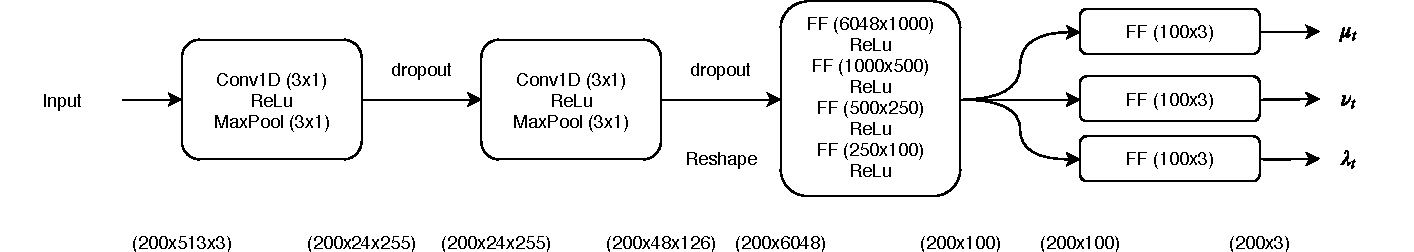
\includegraphics[width=\linewidth]{mirage/cnn.pdf}
    \end{sidecaption}
\end{figure}

\mynewline
As shown in~\cref{fig:mirage:cnn}, it consists of two convolutional modules made of a one-dimensional convolutional layer (1DConv) followed by max-pooling along the frequencies, followed by rectified linear unit (ReLu) activation function and batch-normalization.
The second part consists of a cascade of fully connected feed-forward (FF) layers.
Note that the input dimension is re-arranged so that the second dimension is considered a channel for the 1DConv.
After each layer a dropout probability $p_\text{do} = 0.3$ is applied.

\mynewline
In the \ac{DNN} model presented above, the output consisted only in the time delay $V$.
However, to build a local angular spectrum,
suitable for the \ac{SRP-PHAT}-like algorithm, both means and variances are needed.
Rather than identify these variances with the prediction errors, we explicitly modify the \ac{DNN} model to estimated them\sidenote{
    This idea is similar to the one proposed by Bishop in \ac{MDN} in \citeonly{bishop1994mixture}
    where the output of a neural network parametrizes a Gaussian mixture model.
}.
The main idea behind this design choice is that the learning model can assess its prediction quality.
This approach can be related to existing (Bayesian) data-fusion frameworks, but this direction wav not considered in this work.
\newcommand{\setTDOA}{\ensuremath{\set{\mathtt{TDOA}, \mathtt{iTDOA}, \mathtt{TDOE}}}}
\\To this end, we modify the output of the network to output mean and variances, namely
$V_{\calN} = \set{\mu_{\tau_t}, \sigma^2_{\tau_t}}$
for $t = \setTDOA$.
Moreover, we assume that conditional probability of observing the one of the \ac{TDOA} $\tau_t$ for $t \in \setTDOA$ given the observation $\xi$ in the batch $\Xi$, follows a Gaussian distribution, namely
\begin{equation}
    p(\tau_t \mid  \Xi ; \theta) \sim \calN\kparen{\mu_{\tau_t}(\xi_b;\theta), \sigma^2_{\tau_t}(\xi_b;\theta)}
\end{equation}
where the variance
and the the training loss function
 of~\cref{eq:mirage:mlploss}
\begin{equation}\label{subsec:mirage:mlpcost}
    \calL(V, \hat{V)} = \frac{1}{3} \sum_{b}  \powerOf{\tau_{\mathtt{TDOA}, b} - \hat{\tau}_{\mathtt{TDOA}, b}}
                                            + \powerOf{\tau_{\mathtt{iTDOA}, b} - \hat{\tau}_{\mathtt{iTDOA}, b}}
                                            + \powerOf{\tau_{\mathtt{TDOE}, b} - \hat{\tau}_{\mathtt{TDOE}, b}}
\end{equation}




\newthought{The proposed novel loss function} is the negative Student-T log-likelihood, which is implemented as follows:

\begin{equation}
\begin{split}
\mathcal{L}(\Theta) =& \sum_{x \in B} \sum_{t \in V}\ \dfrac{1}{2} \log (\nu_t\pi_t)
                        + \dfrac{1}{2} \log(\lambda_t^2)
                        - \log  \Gamma \left( \dfrac{\nu_t+1}{2} \right)\\
                    &    + \log  \Gamma \left( \dfrac{\nu_t}{2} \right)
                        + \dfrac{\nu_t+1}{2}
                        \log \left( 1  + \dfrac{\norm{\mu_t, x_i)}}{\nu_t \lambda_t^2} \right)\\
\end{split}
\end{equation}

where $\Theta$ are the CNN parameters and $\Gamma$ is the Gamma function. The summation over $i$ corresponds to the sum among of all the sample $x$ of the batch $B$. and the summation over $t$ corresponds to the sum among the three quantities in V (TDOA, iTDOA, TDOE). It follows that for each each input the network will return the parameters of 3 Student-T distribution ($\mu_t, \nu_t, \lambda_t$) for each variable $t = { \text{TDOA}, \text{iTDOA}, \text{TDOE} }$. Hereafter we denote with $V_{\mathcal{ST}}$ the set of the 9 network outputs.

We use the Adam optimizer ant the normalized root mean square error (nRMSE) is taken as validation metric (see Section~\ref{subsec:eval_synth_tdoa}). The network is manually tuned on a validation set to find the best combination of number of hidden layers and their sizes

Once an estimate $\hat{V_\mathcal{ST}}$ of the parameters of the 3 distribution is returned by the CNN, they are converted to synthetic local angular spectra and passed to an SRP-PHAT method together with the relative positions of true and image microphones which are assumed known. We call this algorithm MIRAGE. The synthetic local angular spectra consist of Student-t distribution with parameters $\mu, \nu$ and $\lambda$.

\begin{table}[ht!]
    \begin{sidecaption}[Echo estimation with MIRAGE results]{%
        \ac{nRMSE} for TDOA estimation and mean angular error in ${}^\circ$ (with accuracies ($\%$))
        for AOA estimation with $\ang{10}$ and $\ang{20}$ angular tolerance.
    }[tab:mirage:tdoas-aoa]
    \centering
    \small
    %\scriptsize
    \begin{tabular*}{\linewidth}{@{\extracolsep{\fill}}cl|ccc|cc@{}}
    \toprule
                &         &          & nRMSE        &                   &\multicolumn{2}{c}{ACCURACY}  \\
                & Input   &    \scriptsize{TDOA}  	&   \scriptsize{iTDOA} 		 &     \scriptsize{TDOE} 		 & $\theta<\ang{10}$ &  $\theta<\ang{20}$ \\
    \midrule
    MIRAGE      &   wn    & 0.18    & 0.28  & 0.25 	& 4.10 (77)	& 5.97 (97) \\
    MIRAGE      &   wn+n  & 0.68    & 0.69  & 0.89 	& 5.00 (26)	& 9.89 (54) \\
    MIRAGE      &   sp    & 0.31    & 0.34  & 0.56  & 4.83 (63)	& 7.26 (82) \\
    MIRAGE      &   sp+n  & 0.99    & 0.98  & 1.48 	& 4.60 (16)	& 9.88 (35) \\
    GCC-PHAT    &   wn    & 0.21    & -     & -		& 4.22 (81) & 6.19 (97) \\
    GCC-PHAT    &   wn+n  & 0.68    & -     & -		& 4.03 (65) & 5.34 (83) \\
    GCC-PHAT    &   sp 	  & 0.32    & -     & -		& 4.08 (82) & 5.34 (97) \\
    GCC-PHAT    &   sp+n  & 1.38    & -     & -		& 4.70 (19) & 8.38 (32) \\
    \bottomrule
    \end{tabular*}
    \end{sidecaption}
\end{table}
